\documentclass[
  captions=tableheading,
  bibliography=totoc, 
  titepage=firstiscover,
]{scrartcl}

\usepackage{blindtext} %neuer input

\usepackage{longtable} % Tabellen über mehrere Seiten

\usepackage[utf8]{inputenc} %neuer input

\usepackage{scrhack}

\usepackage[aux]{rerunfilecheck} %Warnung falls nochmal kompiliert werden muss

\usepackage{fontspec} %Fonteinstellungen

\recalctypearea{}

\usepackage[main=ngerman]{babel} %deutsche Spracheinstellung

\usepackage{ragged2e} %neuer input

\usepackage{amsmath, nccmath}

\usepackage{amssymb} %viele mathe Symbole

\usepackage{mathtools} %Erweiterungen für amsmath


\DeclarePairedDelimiter{\abs}{\lvert}{\rvert}
\DeclarePairedDelimiter{\norm}{\lVert}{\rVert}

\DeclarePairedDelimiter{\bra}{\langle}{\rvert}
\DeclarePairedDelimiter{\ket}{\lvert}{\rangle}

\DeclarePairedDelimiterX{\braket}[2]{\langle}{\rangle}{
#1 \delimsize| #2
}

\NewDocumentCommand \dif {m}
{
\mathinner{\symup{d} #1}
}


\usepackage[
  math-style=ISO,
  bold-style=ISO,
  sans-style=italic,
  nabla=upright,
  partial=upright,
  warnings-off={
    mathtools-colon,
    mathtools-overbracket,
  },
]{unicode-math}

\setmathfont{Latin Modern Math}
\setmathfont{XITS Math}[range={scr, bfscr}]
\setmathfont{XITS Math}[range={cal, bfcal}, StylisticSet=1]


\usepackage[
  locale=DE,
  separate-uncertainty=true,
  per-mode=reciprocal,
  output-decimal-marker={,},
]{siunitx}

\usepackage[autostyle]{csquotes} %richtige Anführungszeichen

\usepackage{xfrac}

\usepackage{float}

\floatplacement{figure}{htbp}

\floatplacement{table}{htbp}

\usepackage[ %floats innerhalb einer section halten
  section,   %floats innerhalb er section halten
  below,     %unterhalb der Section aber auf der selben Seite ist ok
]{placeins}

\usepackage[
  labelfont=bf,
  font=small,
  width=0.9\textwidth,
]{caption}

\usepackage{subcaption} %subfigure, subtable, subref

\usepackage{graphicx}

\usepackage{grffile}

\usepackage{booktabs}

\usepackage{microtype} %Verbesserungen am Schriftbild

\usepackage[
backend=biber,
]{biblatex}

\addbibresource{../lit.bib}

\usepackage[ %Hyperlinks im Dokument
  german,
  unicode,
  pdfusetitle,
  pdfcreator={},
  pdfproducer={},
]{hyperref}

\usepackage{bookmark}

\usepackage[shortcuts]{extdash}

%\usepackage{warpcol}


\begin{document}
    \title{ATP Übungsblatt 8}
    \author{  
    Tobias Rücker\\
    \texorpdfstring{\href{mailto:tobias.ruecker@tu-dortmund.de}{tobias.ruecker@tu-dortmund.de}
    \and}{,} 
    Paul Störbrock\\
    \texorpdfstring{\href{mailto:paul.stoerbrock@tu-dortmund.de}{paul.stoerbrock@tu-dortmund.de}}{}
    }
\maketitle
\center{\Large Abgabegruppe: \textbf{Mittw. 10-12 Uhr}}
\thispagestyle{empty}

\newpage
\tableofcontents
\thispagestyle{empty}
\newpage

\setcounter{page}{1}


\section{Aufgabe 22}

    \begin{figure}[H]
        \centering
        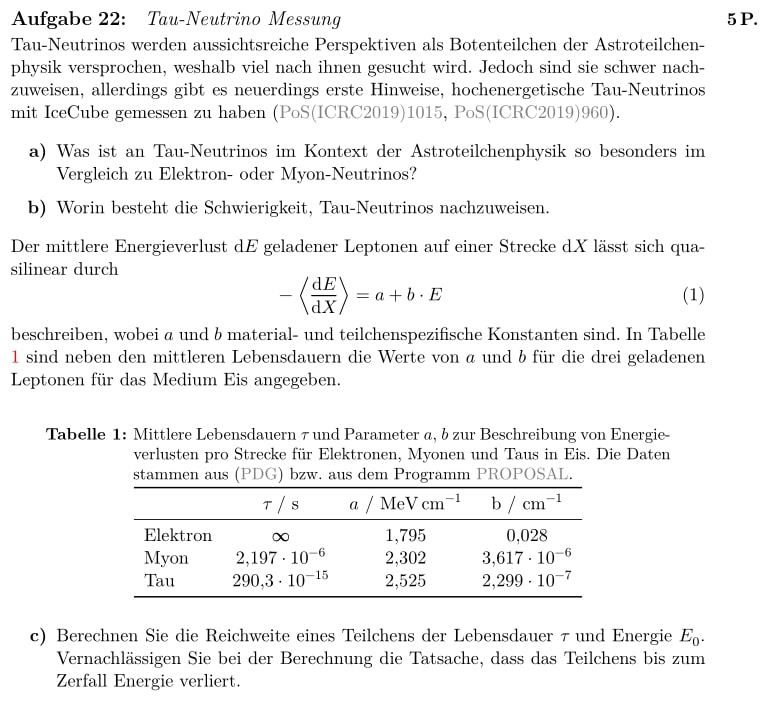
\includegraphics[width=\textwidth]{images/Aufgabe22a.jpg}
        \label{fig:1}
    \end{figure}

    \begin{figure}[H]
        \centering
        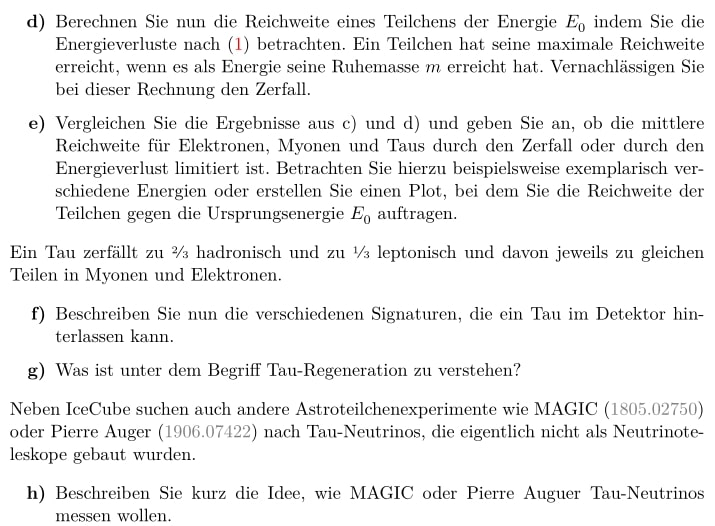
\includegraphics[width=\textwidth]{images/Aufgabe22b.jpg}
        \label{fig:2}
    \end{figure}

\subsection{a)}

    Eine der Besonderheiten der Tau-Neutrinos ist, dass sein erzeugendes Teilchen ,das Tau ,sehr schnell zerfällt
    , wohingegen Elektronen beim durchqueren der Erde absorbiert werden und Myonen all 
    ihre Energie verlieren und dann ein Neutrino erzeugen, dass zu energiearm ist um gemessen zu werden.
    Das Tau hingegen erzeugt ein hochenergetisches Tau-Neutrino. Je höher die Energie ist
    desto wahrscheinlicher wechselwirkt das Teilchen, was vorteilhaft für Messungen an
    Detektoren sind. Zudem können die Taus aufgrund der Tau-Regeneration durch die Erde propagieren
    und immer noch gemessen werden von Detektoren wie dem ice-cube.

\subsection{b)}
Ein Nachteil für die Messungen ist, dass immer nur ein kleiner Teil des Himmels
abesucht werden kann und es zu viele atmosphärische Signale gibt

\subsection{c)}
    Definition:\\
    $E$: Ruheenergie\\
    $E_0$: Gesamtenergie
    \begin{align}
        E_0 &= \gamma E \Leftrightarrow \gamma = \frac{E_0}{E}\\
        m &= \gamma m\\
        \tau &= \gamma \tau_0 \qquad \gamma\; \text{einsetzen}\\
        &= \frac{E_0}{E} \tau_0\\
        r &= v\tau_0\\
        v &= \frac{mv}{m} = \frac{p}{mc^2}c^2 = \frac{p}{E_0}c^2\\
        E_0^2 &= E^2 + (cp)^2 \Leftrightarrow p = \frac{\sqrt{E_0^2-E^2}}{E_0} \qquad \text{einsetzten in $v$}\\
        \Rightarrow v &= \frac{\sqrt{E_0^2-E^2}}{E_0}c \qquad \text{einsetzten in $r$}\\
        \\
        \Rightarrow r &= \frac{\sqrt{E_0^2-E^2}}{E_0} \frac{E_0}{E} \tau_0 c\\
        &= \frac{\sqrt{E_0^2-E^2}}{m_0 c^2} \tau_0 c\\
        &= \frac{\sqrt{E_0^2-E^2}}{m_0 c} \tau_0
    \end{align}

\subsection{d)}

    \begin{align}
        -\int_{E_0}^{E} \frac{1}{(a+bE')} \mathrm{d}E' &= \int_{0}^{1} 1 \mathrm{d}x\\
        -\frac{1}{b}\log(a+bE')\vert_{e_0}^{E} &= r\\
        r_{\langle \frac{\mathrm{d}E}{\mathrm{d}x} \rangle} &= -\frac{1}{b}\log\left(\frac{a+bE}{a+bE_0}\right)
    \end{align}

\subsection{e)}


\begin{figure}[H]
    \centering
    \includegraphics[width=\textwidth]{plot_c.pdf}
    \caption{Reichweite in c) gegen die Energie aufgetragen(Für ein Myon)}
\end{figure}


\begin{figure}[H]
    \centering
    \includegraphics[width=\textwidth]{plot_d.pdf}
    \caption{Reichweite in d) gegen die Energie aufgetragen(für ein Myon)}
\end{figure}


\subsection{f)}
Ein Tau kann im Detektor einen Doppelimpuls hinterlassen, dabei stammt ein Puls
aus einem hadronischem und der andere aus einem leptonischen Zerfall.

\subsection{g)}
Die Tau-Regenartion beschreibt einen Prozess, bei dem ein Tau-Neutrino in ein
Tau umgewandelt ist, dass sehr energiereich ist. Dadurch zerfällt es schnell
in ein Tau-Neutrino und dieser Prozess wiederholt sich. Bei jedem Schritt 
verliert es etwas Energie dabei.

\subsection{h)}


\section{Aufgabe 23}

    \begin{figure}[H]
        \centering
        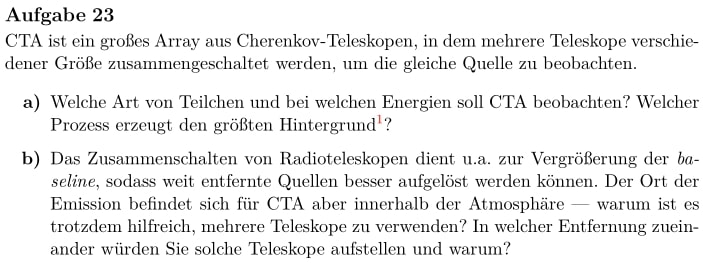
\includegraphics[width=\textwidth]{images/Aufgabe23a.jpg}
        \label{fig:3}
    \end{figure}

    \begin{figure}[H]
        \centering
        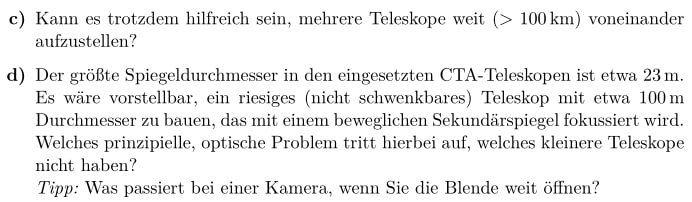
\includegraphics[width=\textwidth]{images/Aufgabe23b.jpg}
        \label{fig:4}
    \end{figure}

\subsection{a)}

    \flushleft{Das\;}\justifying Cherenkov Telescope Array (CTA) such nach elektromagentischen Schauern, die von hochenergetischen
    Photone verursacht werden. Das dabei entstehende Cherenkovlicht kann von dem Array gemessen werden.\\
    Der Messbereich des CTAs liegt bei ca. \SI{10}{\giga\electronvolt} bis \SI{100}{\tera\electronvolt}.\\
    Hadronen-Schauer stellen den größten Hintergrund da, da diese ca. 10000-mal häufiger auftreten, als 
    elektromagentische Schauer.

\subsection{b)}

    \flushleft{Es\;}\justifying ist durchaus hilfreich Radioteleskope bei einer Messung innerhalb der Atmosphäre 
    zusammenzuschalten, da so stereoskopische Messungen möglich sind. Es kann also der Ursprung des Schauers bestimmt
    werden. Der Abstand der Teleskope sollte so gewählt werden, dass möglichst viele innerhalb des Schauerfußabdrucks 
    liegen. Da der Fußabdruck einen Druchmesser von ca. \SI{300}{\meter} hat, sollten die Teleskope mit einem Abstand von unter
    \SI{150}{\meter} in grid-formation aufgestellt werden, da so mit ein wenig Glück vier Teleskope innerhalb des light pools
    stehen und eine stereoskopische Beobachtung ermöglichen. Dadurch kann die Position der Quelle bestimmt werden. 

\subsection{c)}

    \flushleft{Ja,\;}\justifying zum Beispiel Imaging Atmospheric Cherenkov Telescopes (IACTs) messen das Cherenkovlicht, welches in der 
    Atmosphäre auftritt. Demnach ist die Atmosphäre das Detektionsmedium, wodurch die Fläche, welche die IACTs beobachten müssen, sehr groß
    wird. Also macht es Sinn, die Teleskope möglichst weit auseinander aufzustellen.  

\subsection{d)}

    \flushleft{Das\;}\justifying Messen weiterer Ereignisse ist auf der einen Seite das Ziel, kann aber bei einem einzelnen Teleskop zu Schwierigkeiten
    führen. Bei einer größeren Fläche steigen die gemessen Ereignisse quadratisch an. Gleichermaßen steigt aber auch der Hintergrund quadratisch an. 
    Das dabei enstehende Problem ist die Aufzeichnung der Messdaten. Die Photomultiplier würden überlastet werden und an Genauigkeit verlieren. Die
    Technik für die Datenverarbeitung würde deutlich teuerer werden, ebenso die Herstellung der großen Spiegel, da diese immens präzise geschliffen werden 
    müssen um eine adäquate Genauigkeit zu erzielen. 

\section{Aufgabe 24}

    \begin{figure}[H]
        \centering
        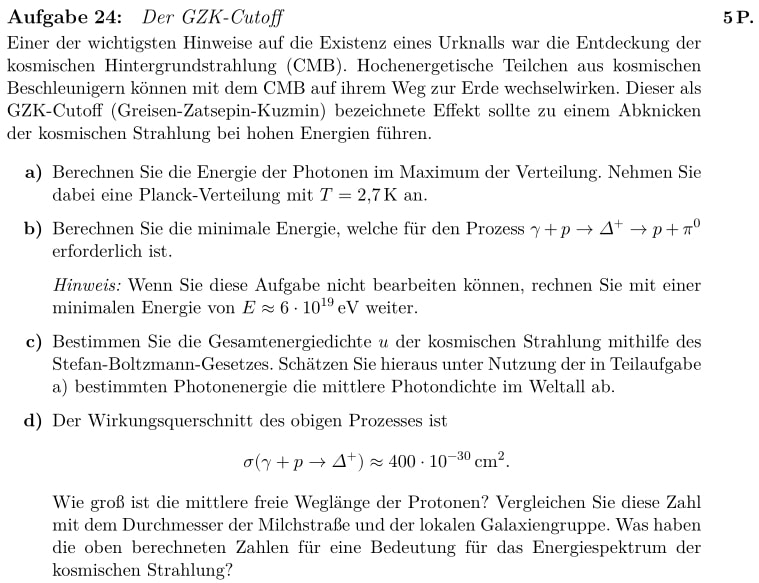
\includegraphics[width=\textwidth]{images/Aufgabe24.jpg}
        \label{fig:5}
    \end{figure}

\subsection{a)}

\subsection{b)}

\subsection{c)}

\subsection{d)}

\end{document}